\documentclass[tikz,border=6pt]{standalone}
% Shared style for the HERMESS schematic figures (compiled by build.sh).
% ETH palette; Latin Modern (the LaTeX default) to match the documentation.
\usepackage{amsmath}
\usepackage{tikz}
\usetikzlibrary{arrows.meta,positioning,calc,shapes.geometric,circuits.ee.IEC}
\definecolor{ethblue}{HTML}{215CAF}
\definecolor{ethpetrol}{HTML}{007894}
\definecolor{ethgrey}{HTML}{6F6F6F}
\tikzset{
  block/.style      = {draw=ethblue, thick, fill=ethblue!8, minimum height=9mm,
                       minimum width=16mm, inner sep=2.5pt, align=center},
  sum/.style        = {draw=ethblue, thick, circle, fill=white, minimum size=4.5mm, inner sep=0pt},
  sig/.style        = {-{Latex[length=2.4mm]}, thick},
  wire/.style       = {thick},
  node distance     = 9mm and 12mm,
  every node/.style = {font=\small},
  lbl/.style        = {font=\small, inner sep=1.5pt},
  port/.style       = {font=\small\itshape, text=ethgrey},
}

\usetikzlibrary{decorations.pathmorphing}
\tikzset{spring/.style={thick, decorate, decoration={coil, aspect=0.6, segment length=2.0mm, amplitude=1.6mm, pre length=2mm, post length=2mm}}}
\begin{document}
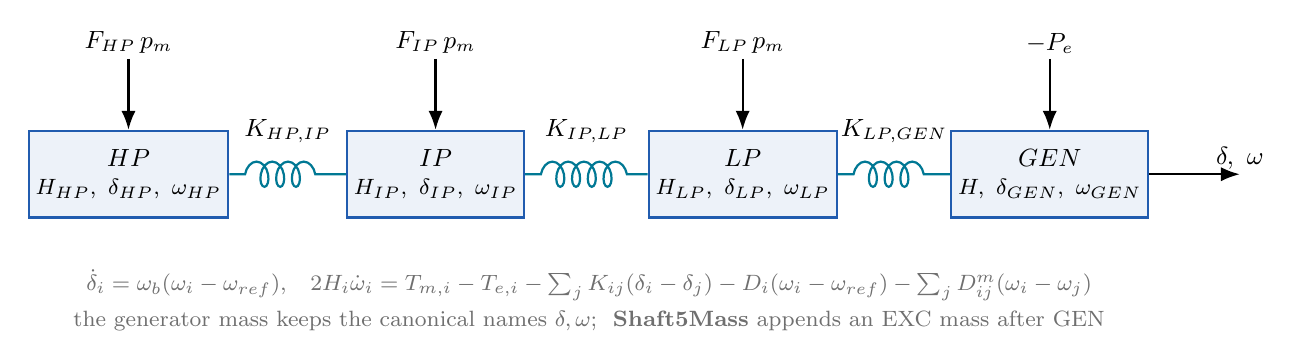
\begin{tikzpicture}
  \foreach \x/\n/\h in {0/HP/{H_{HP}}, 3.9/IP/{H_{IP}}, 7.8/LP/{H_{LP}}, 11.7/GEN/{H}} {
    \node[block, minimum width=17mm, minimum height=11mm, align=center] (\n) at (\x,0) {$\n$\\[-1pt]{\footnotesize $\h,\ \delta_{\n},\ \omega_{\n}$}};
  }
  \draw[spring, ethpetrol] (HP.east) -- (IP.west);
  \node[lbl] at ($(HP.east)!0.5!(IP.west)+(0,0.55)$) {$K_{HP,IP}$};
  \draw[spring, ethpetrol] (IP.east) -- (LP.west);
  \node[lbl] at ($(IP.east)!0.5!(LP.west)+(0,0.55)$) {$K_{IP,LP}$};
  \draw[spring, ethpetrol] (LP.east) -- (GEN.west);
  \node[lbl] at ($(LP.east)!0.5!(GEN.west)+(0,0.55)$) {$K_{LP,GEN}$};
  \foreach \n/\f in {HP/{F_{HP}}, IP/{F_{IP}}, LP/{F_{LP}}} {
    \draw[sig] ($(\n.north)+(0,0.9)$) node[above, lbl] {$\f\, p_m$} -- (\n.north);
  }
  \draw[sig] ($(GEN.north)+(0,0.9)$) node[above, lbl] {$-P_e$} -- (GEN.north);
  \draw[sig] (GEN.east) -- ++(1.15,0) node[above, lbl] {$\delta,\ \omega$};
  \node[lbl, text=ethgrey, align=center] at (5.85,-1.6)
    {\footnotesize $\dot{\delta}_i = \omega_b(\omega_i - \omega_{ref})$,\quad
     $2H_i\dot{\omega}_i = T_{m,i} - T_{e,i} - \sum_j K_{ij}(\delta_i - \delta_j) - D_i(\omega_i - \omega_{ref}) - \sum_j D^m_{ij}(\omega_i - \omega_j)$\\[2pt]
     \footnotesize the generator mass keeps the canonical names $\delta, \omega$;\ \ \textbf{Shaft5Mass} appends an EXC mass after GEN};
\end{tikzpicture}
\end{document}
